KisTA enables the export of a TiKZ file, which in turn, can be compiled into an image
which reflects the KisTA model.
%
The export can be enabled and configured both from
the C/C++ API and the KisTA XML front-end.
%
KisTA provides methods for enabling a configuring the exported sketch.
A big advantage of exporting to TiKZ is that it makes possible to perform user specific
editions on TiKZ file, before compiling the sketch image.

\subsubsection{Using C++ API}
\label{sec:sketch_report_cpp_api}

Listing~\ref{list:sketch_report_class} shows the API that the user can use for enabling and controlling the export of a system sketch.

%\begin{table}[t]
\begin{lstlisting}[style=KistaCodeStyle,caption={API for controling tracing tasks and scheduler activity.},label=list:sketch_report_class]

class sketch_report_t : sc_module {
	friend sketch_report_t& operator<<(sketch_report_t& sk_rpt, std::string content);
public:
		// create sketch report class, by default disabled
		// sketch file with the default name "system_sketch"
	sketch_report_t();
	
	bool &is_enabled(); // true if sketch reported enabled
	
		// set name of sketch report file
	void set_file_name(std::string	name_par); 
	
	void enable(); // enable sketch report and creates report header
	                // (has to be called at construction time and after set_name, otherwise, settled name is overriden and the default one taken)
	
	// configuration of the draw
	void draw_sys_level_conn();
	
	void highlight_environment();
	void highlight_system();      // overrides the hilighting of application and platform
	void highlight_application();
	void highlight_platform();

        void only_image();
        void set_scale(float scale_par);

   ...
};

\end{lstlisting}
%\end{table}

When the user includes the "kista.h" header, a global element \texttt{sketch\_report} of type \texttt{sketch\_report\_t}
is immediately instanced.

In the simplest case, the user only needs to call the \texttt{enable()} method, before the \texttt{sc\_start()} method.
Then, to generate the sketch, to lauch the KisTA executable is necessary.
The sketch is generated at the end of the elaboration.
Therefore, it is not necessary to run the simulation phase (call to \texttt{sc\_start}) to generate the sketch report.

By default, the file is generated with the name \texttt{system\_sketch.tex}.
The user can control the name of the sketch by means of the \texttt{set\_file\_name} method,
which has to be called before the call to the \texttt{enable()} method.

The method \texttt{is\_enabled()} serves to test if the sketch has been enabled.

Figure~\ref{fig:ex3_sketch} ilustrates the result of the sketch reported
after applying the \texttt{pdflatex} command to the \texttt{ex3\_sketch.tex} file
produced in the basic real-time example 3.
This example consists of two independent tasks mapped to a single local scheduler.
Notice that the reported sketch represents the default processing element
instanced by KisTA when the user does not explicitly specifies a processing element.
%

\begin{figure}[h]
\centering
%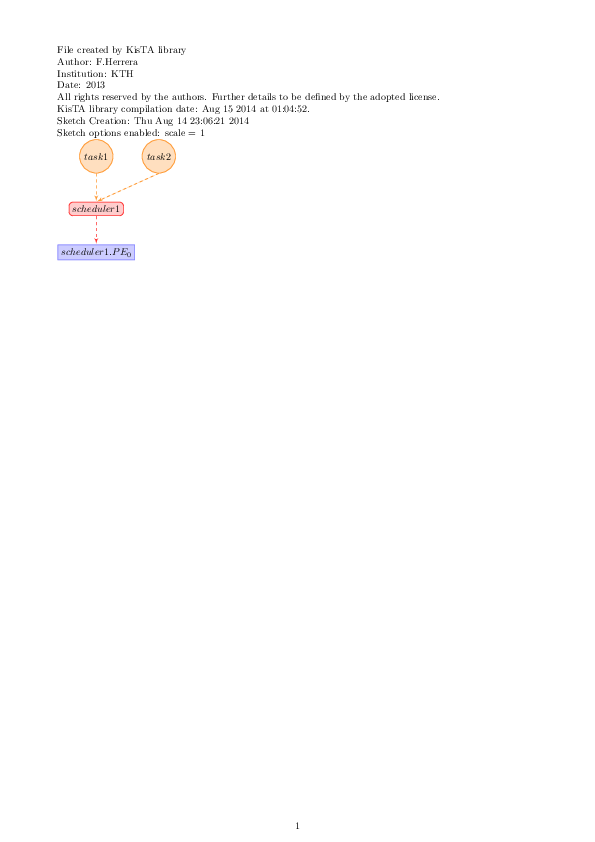
\includegraphics[width=\textwidth]{./figs/ex3_sketch.png} 
\fbox{
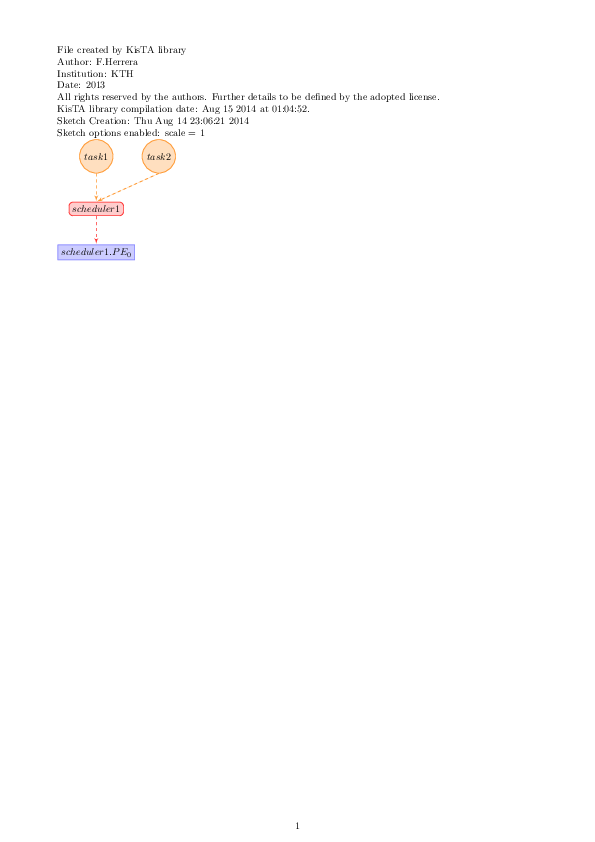
\includegraphics[width=0.75\textwidth]{./figs/ex3_sketch.png} 
}
\caption{Sketch report of basic RT example 3.} 
\label{fig:ex3_sketch}
\end{figure}

The export is done for an A4 paper format.
A text with information about the options, date, etc used for producing the report is first included
by default.
The \texttt{only\_image()} method can be used for avoiding such textual report
associated to the image.
%
This can be used together with the method \texttt{set\_scale(float)} in order to 
generate a pdf image taking most of the paper size, and to reduce the need
for further transformations when converting to other formats.

Listing~\ref{list:sketch_commands_ex3} shows 
an excerpt of basic RT example 3, using \texttt{only\_image()} and \texttt{set\_scale(4.0)},
as an example of utilization of configuration commands to export only an image with a x4 scaling.

%
After compiling the KisTA executable, and running it, the result
is a file called \texttt{ex3\_sketch.tex}.
%
Running the \texttt{pdflatex} command on this file produces the result
of Figure~\ref{fig:ex3_sketch_only_img}.

%\begin{table}[t]
\begin{lstlisting}[style=KistaCodeStyle,caption={Commands controling sketch report in basic RT example 3.},label=list:sketch_commands_ex3]

  ...
  sketch_report.set_file_name("ex3_sketch"); 

  sketch_report.enable();
   
  sketch_report.only_image();
   
  sketch_report.set_scale(4.0);
  ...

  sc_start();
  ...
};

\end{lstlisting}
%\end{table}


\begin{figure}[h]
\centering
%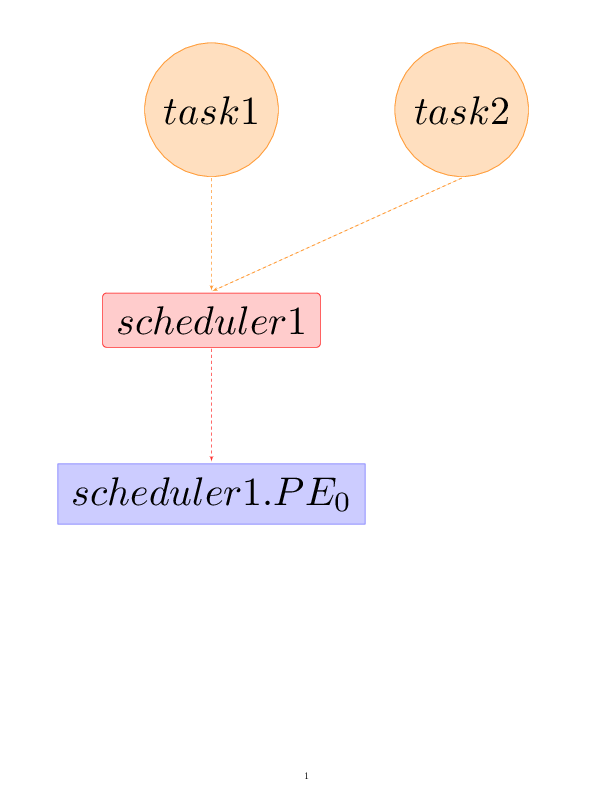
\includegraphics[width=\textwidth]{./figs/ex3_sketch_only_image_scale4.png} 
\fbox{
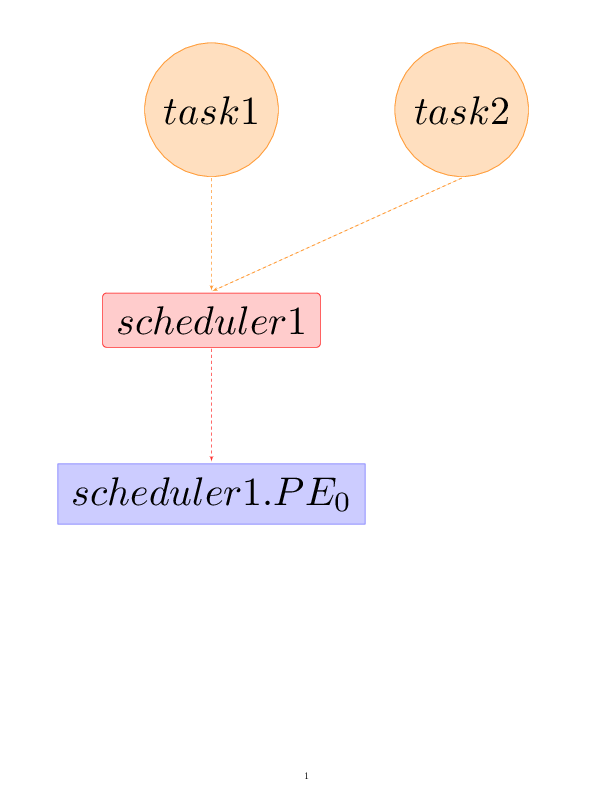
\includegraphics[width=0.75\textwidth]{./figs/ex3_sketch_only_image_scale4.png} 
}
\caption{Sketch report of basic RT example 3, configured to report only the image and with x4 scale} 
\label{fig:ex3_sketch_only_img}
\end{figure}


\subsubsection{Using the XML front-end}
\label{sec:sketch_report_xml}

The sketch report can be also enabled and configured from the XML interface.

The Listing~\ref{list:xml_sketch_1} shows a first configuration example where
the sketch report is enabled for the void activity detection (VAD) example.
In addition, the name of the text file is configured to be \texttt{vad\_sketch.tex}.
Figure~\ref{fig:vad_sketch_1} shows the result of the configuration.
The sketch, by default, as well as the application tasks and their system-level 
communications, include the environment tasks (in an upper level), the I/O connections,
and also the platform elements and the mappings.

%\begin{table}[t]
\begin{lstlisting}[language=XML, caption={Configuring sketch report from the XML interface.}, label=list:xml_sketch_1]
<kista_configuration>
   ...
   <export_sketch value="true">
      <file_name value="vad_sketch"/>
      <draw_sys_level_conn_names value="true"/>
      <highlight_platform value="true"/>
   </export_sketch>	
   ...
</kista_configuration>
\end{lstlisting}

The Listing~\ref{list:xml_sketch_1} also shows 
that it is necessary to explicitly enable the drawing of the names 
of the system-level connections, and also the configuration to highlight 
the platform elements (including the SW platform and the HW platform).

\begin{figure}[h]
\centering
%\includegraphics[width=\textwidth]{./figs/.png} 
\fbox{
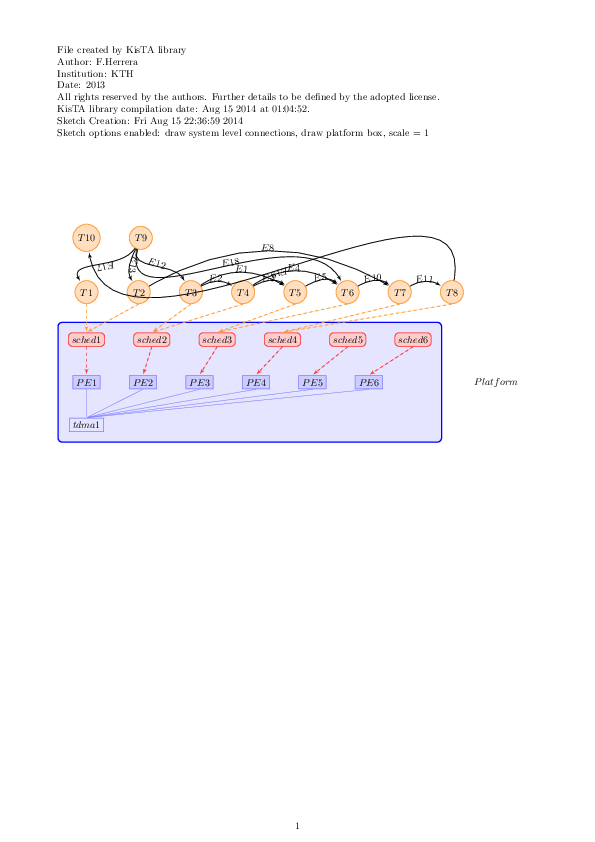
\includegraphics[width=0.75\textwidth]{./figs/vad_sketch_1.png} 
}
\caption{Sketch report of VAD example where the names of the system-level connections are drawn too.} 
\label{fig:vad_sketch_1}
\end{figure}

The Listing~\ref{list:xml_sketch_2} shows a variant where the environment and the systems 
are separately highlighted.
The resulting sketch is shown in Figure~\ref{fig:vad_sketch_2}.

%\begin{table}[t]
\begin{lstlisting}[language=XML, caption={Hilighting the environment and the system from the XML interface.}, label=list:xml_sketch_2]
<kista_configuration>
   ...
   <export_sketch value="true">
      <file_name value="vad_sketch"/>
      <draw_sys_level_conn_names value="true"/>
      <highlight_environment value="true"/>
      <highlight_system value="true"/>
   </export_sketch>	
   ...
</kista_configuration>
\end{lstlisting}

\begin{figure}[h]
\centering
%\includegraphics[width=\textwidth]{./figs/.png} 
\fbox{
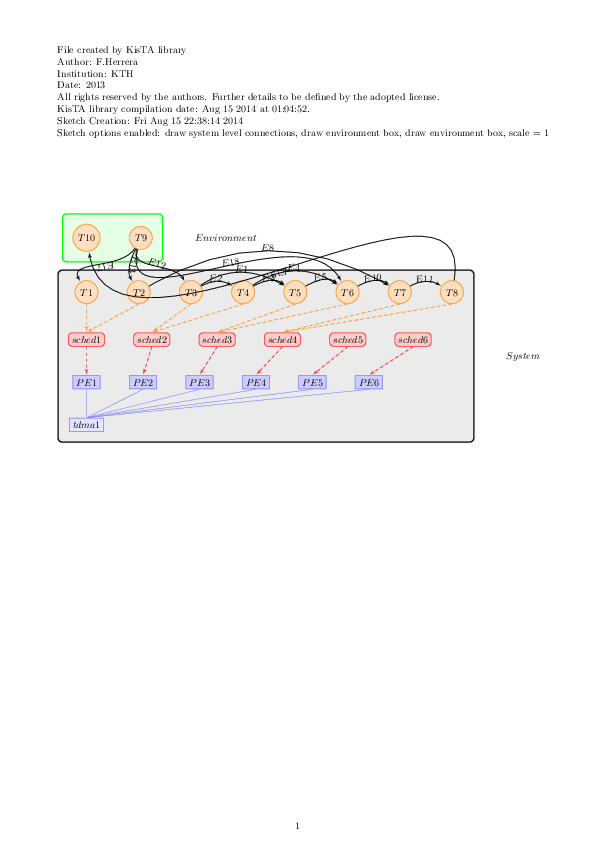
\includegraphics[width=0.75\textwidth]{./figs/vad_sketch_2.png} 
}
\caption{Sketch report of the VAD example with system and environment highlighting-} 
\label{fig:vad_sketch_2}
\end{figure}


The Listing~\ref{list:xml_sketch_3} shows a variant whitout any highlighting, and 
configure to only export the image and scaling up 25\% the original size.
The resulting sketch is shown in Figure~\ref{fig:vad_sketch_only_img_1_25}.

%\begin{table}[t]
\begin{lstlisting}[language=XML, caption={Configuring and only image sketch and its scale from the XML interface.}, label=list:xml_sketch_3]
<kista_configuration>
   ...
   <export_sketch value="true">
      <file_name value="vad_sketch"/>
      <draw_sys_level_conn_names value="true"/>
      <only_image value="true"/>
      <set_scale value="1.25"/>
   </export_sketch>	
   ...
</kista_configuration>
\end{lstlisting}

\begin{figure}[h]
\centering
%\includegraphics[width=\textwidth]{./figs/.png} 
\fbox{
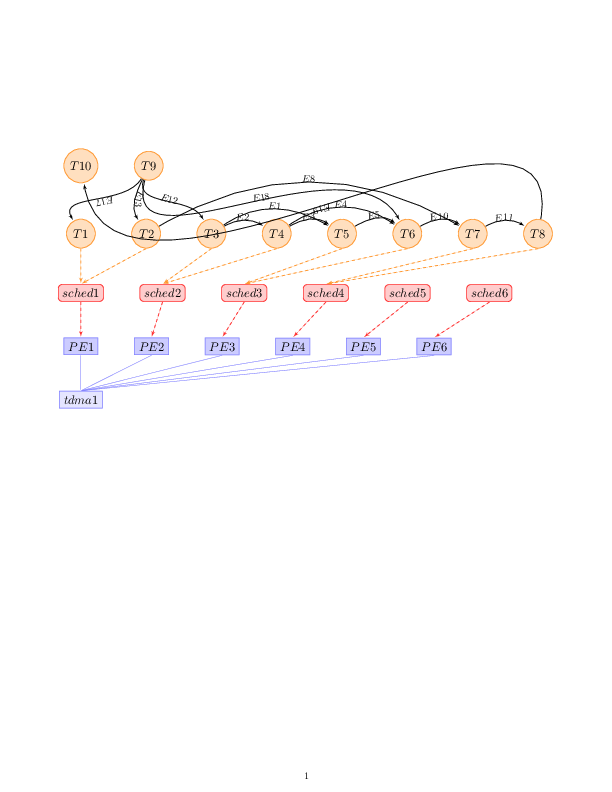
\includegraphics[width=0.75\textwidth]{./figs/vad_sketch_only_img_1_25.png} 
}
\caption{Only image sketch report of the VAD example and with scale=1.25} 
\label{fig:vad_sketch_only_img_1_25}
\end{figure}

